\documentclass[11pt]{article}

% This first part of the file is called the PREAMBLE. It includes
% customizations and command definitions. The preamble is everything
% between \documentclass and \begin{document}.

\usepackage[margin=0.6in]{geometry} % set the margins to 1in on all sides
\usepackage[demo]{graphicx} % to include figures
\usepackage{amsmath} % great math stuff
\usepackage{amsfonts} % for blackboard bold, etc
\usepackage{amsthm} % better theorem environments
% various theorems, numbered by section
\usepackage{amssymb}
\usepackage[utf8]{inputenc}
\usepackage{booktabs}
\usepackage{array}
\usepackage{courier}
\usepackage[usenames, dvipsnames]{color}
\usepackage{titlesec}
\usepackage{empheq}
\usepackage{tikz}
\usepackage{caption}
\usepackage{subcaption}


\newcommand\encircle[1]{%
  \tikz[baseline=(X.base)] 
    \node (X) [draw, shape=circle, inner sep=0] {\strut #1};}
 
% Command "alignedbox{}{}" for a box within an align environment
% Source: http://www.latex-community.org/forum/viewtopic.php?f=46&t=8144
\newlength\dlf  % Define a new measure, dlf
\newcommand\alignedbox[2]{
% Argument #1 = before & if there were no box (lhs)
% Argument #2 = after & if there were no box (rhs)
&  % Alignment sign of the line
{
\settowidth\dlf{$\displaystyle #1$}  
    % The width of \dlf is the width of the lhs, with a displaystyle font
\addtolength\dlf{\fboxsep+\fboxrule}  
    % Add to it the distance to the box, and the width of the line of the box
\hspace{-\dlf}  
    % Move everything dlf units to the left, so that & #1 #2 is aligned under #1 & #2
\boxed{#1 #2}
    % Put a box around lhs and rhs
}
}


\newtheorem{thm}{Theorem}[section]
\newtheorem{lem}[thm]{Lemma}
\newtheorem{prop}[thm]{Proposition}
\newtheorem{cor}[thm]{Corollary}
\newtheorem{conj}[thm]{Conjecture}

\setcounter{secnumdepth}{4}

\titleformat{\paragraph}
{\normalfont\normalsize\bfseries}{\theparagraph}{1em}{}
\titlespacing*{\paragraph}
{0pt}{3.25ex plus 1ex minus .2ex}{1.5ex plus .2ex}

\definecolor{myblue}{RGB}{72, 165, 226}
\definecolor{myorange}{RGB}{222, 141, 8}

\setlength{\heavyrulewidth}{1.5pt}
\setlength{\abovetopsep}{4pt}


\DeclareMathOperator{\id}{id}
\DeclareMathOperator{\argmin}{\arg\!\min}
\DeclareMathOperator{\Tr}{Tr}

\newcommand{\bd}[1]{\mathbf{#1}} % for bolding symbols
\newcommand{\RR}{\mathbb{R}} % for Real numbers
\newcommand{\ZZ}{\mathbb{Z}} % for Integers
\newcommand{\col}[1]{\left[\begin{matrix} #1 \end{matrix} \right]}
\newcommand{\comb}[2]{\binom{#1^2 + #2^2}{#1+#2}}
\newcommand{\bs}{\boldsymbol}
\newcommand{\opn}{\operatorname}
\begin{document}
\nocite{*}

\title{Testing Performances of Sparse GPVB and Variational Approximation for Linear Mixed Model}

\author{Daeyoung Lim\thanks{Prof. Taeryon Choi} \\
Department of Statistics \\
Korea University}

\maketitle

\section{Performance: GPVB}
  The model was initially
  $$
    y = \mathsf{E}\left[Z\right]\alpha + A\beta + \epsilon.
  $$
  Since we are running mean-field variational approximation, we are updating variational parameters of the optimal distributions, thereby enabling the replacement of each parameter with its variational parameter. Therefore, the fitted model will be
  $$
    \hat{y} = Z\mu_{q\left(\alpha\right)} + A\mu_{q\left(\beta\right)}.
  $$
  However, we should keep in mind that there is $\lambda$ inside $Z$ so we must not forget to replace $\lambda$ with $\mu_{q\left(\lambda\right)}$. With the data obtained from \emph{J. T. Ormerod \& M. P. Wand (2010) Explaining Variational Approximations, The American Statisticians}, we tested the implemented code. By using the \emph{root MSE(RMSE)} defined as follows,
  $$
    \text{RMSE} = \sqrt{\frac{1}{n}\sum_{i=1}^{n}\left(y_{i}-\hat{y}_{i}\right)^{2}},
  $$
  we can test the performances of multiple codes.
  \begin{itemize}
    \item For GPVB, $\text{RMSE}_{\text{GPVB}}= 1.890758$.
    \item For ordinary VB, $\text{RMSE}_{\text{VB}} = 1.961782$.
    \item To test how much the two models differ, though we wish them to be fairly similar, we also consider computing the following measure(\emph{root sum of squared differences}): 
    $$
      \text{RSSD} = \sqrt{\frac{1}{n}\sum_{i=1}^{n}\left(\hat{y}_{\text{GPVB}}-\hat{y}_{\text{VB}} \right)^{2}}.
    $$
    \item $\text{RSSD} = 2.114151$.
  \end{itemize}
\section{GP normal effect}
  We present a simple tutorial on simulation.
  \begin{figure}
    \centering
    \begin{subfigure}{.5\textwidth}
      \centering
      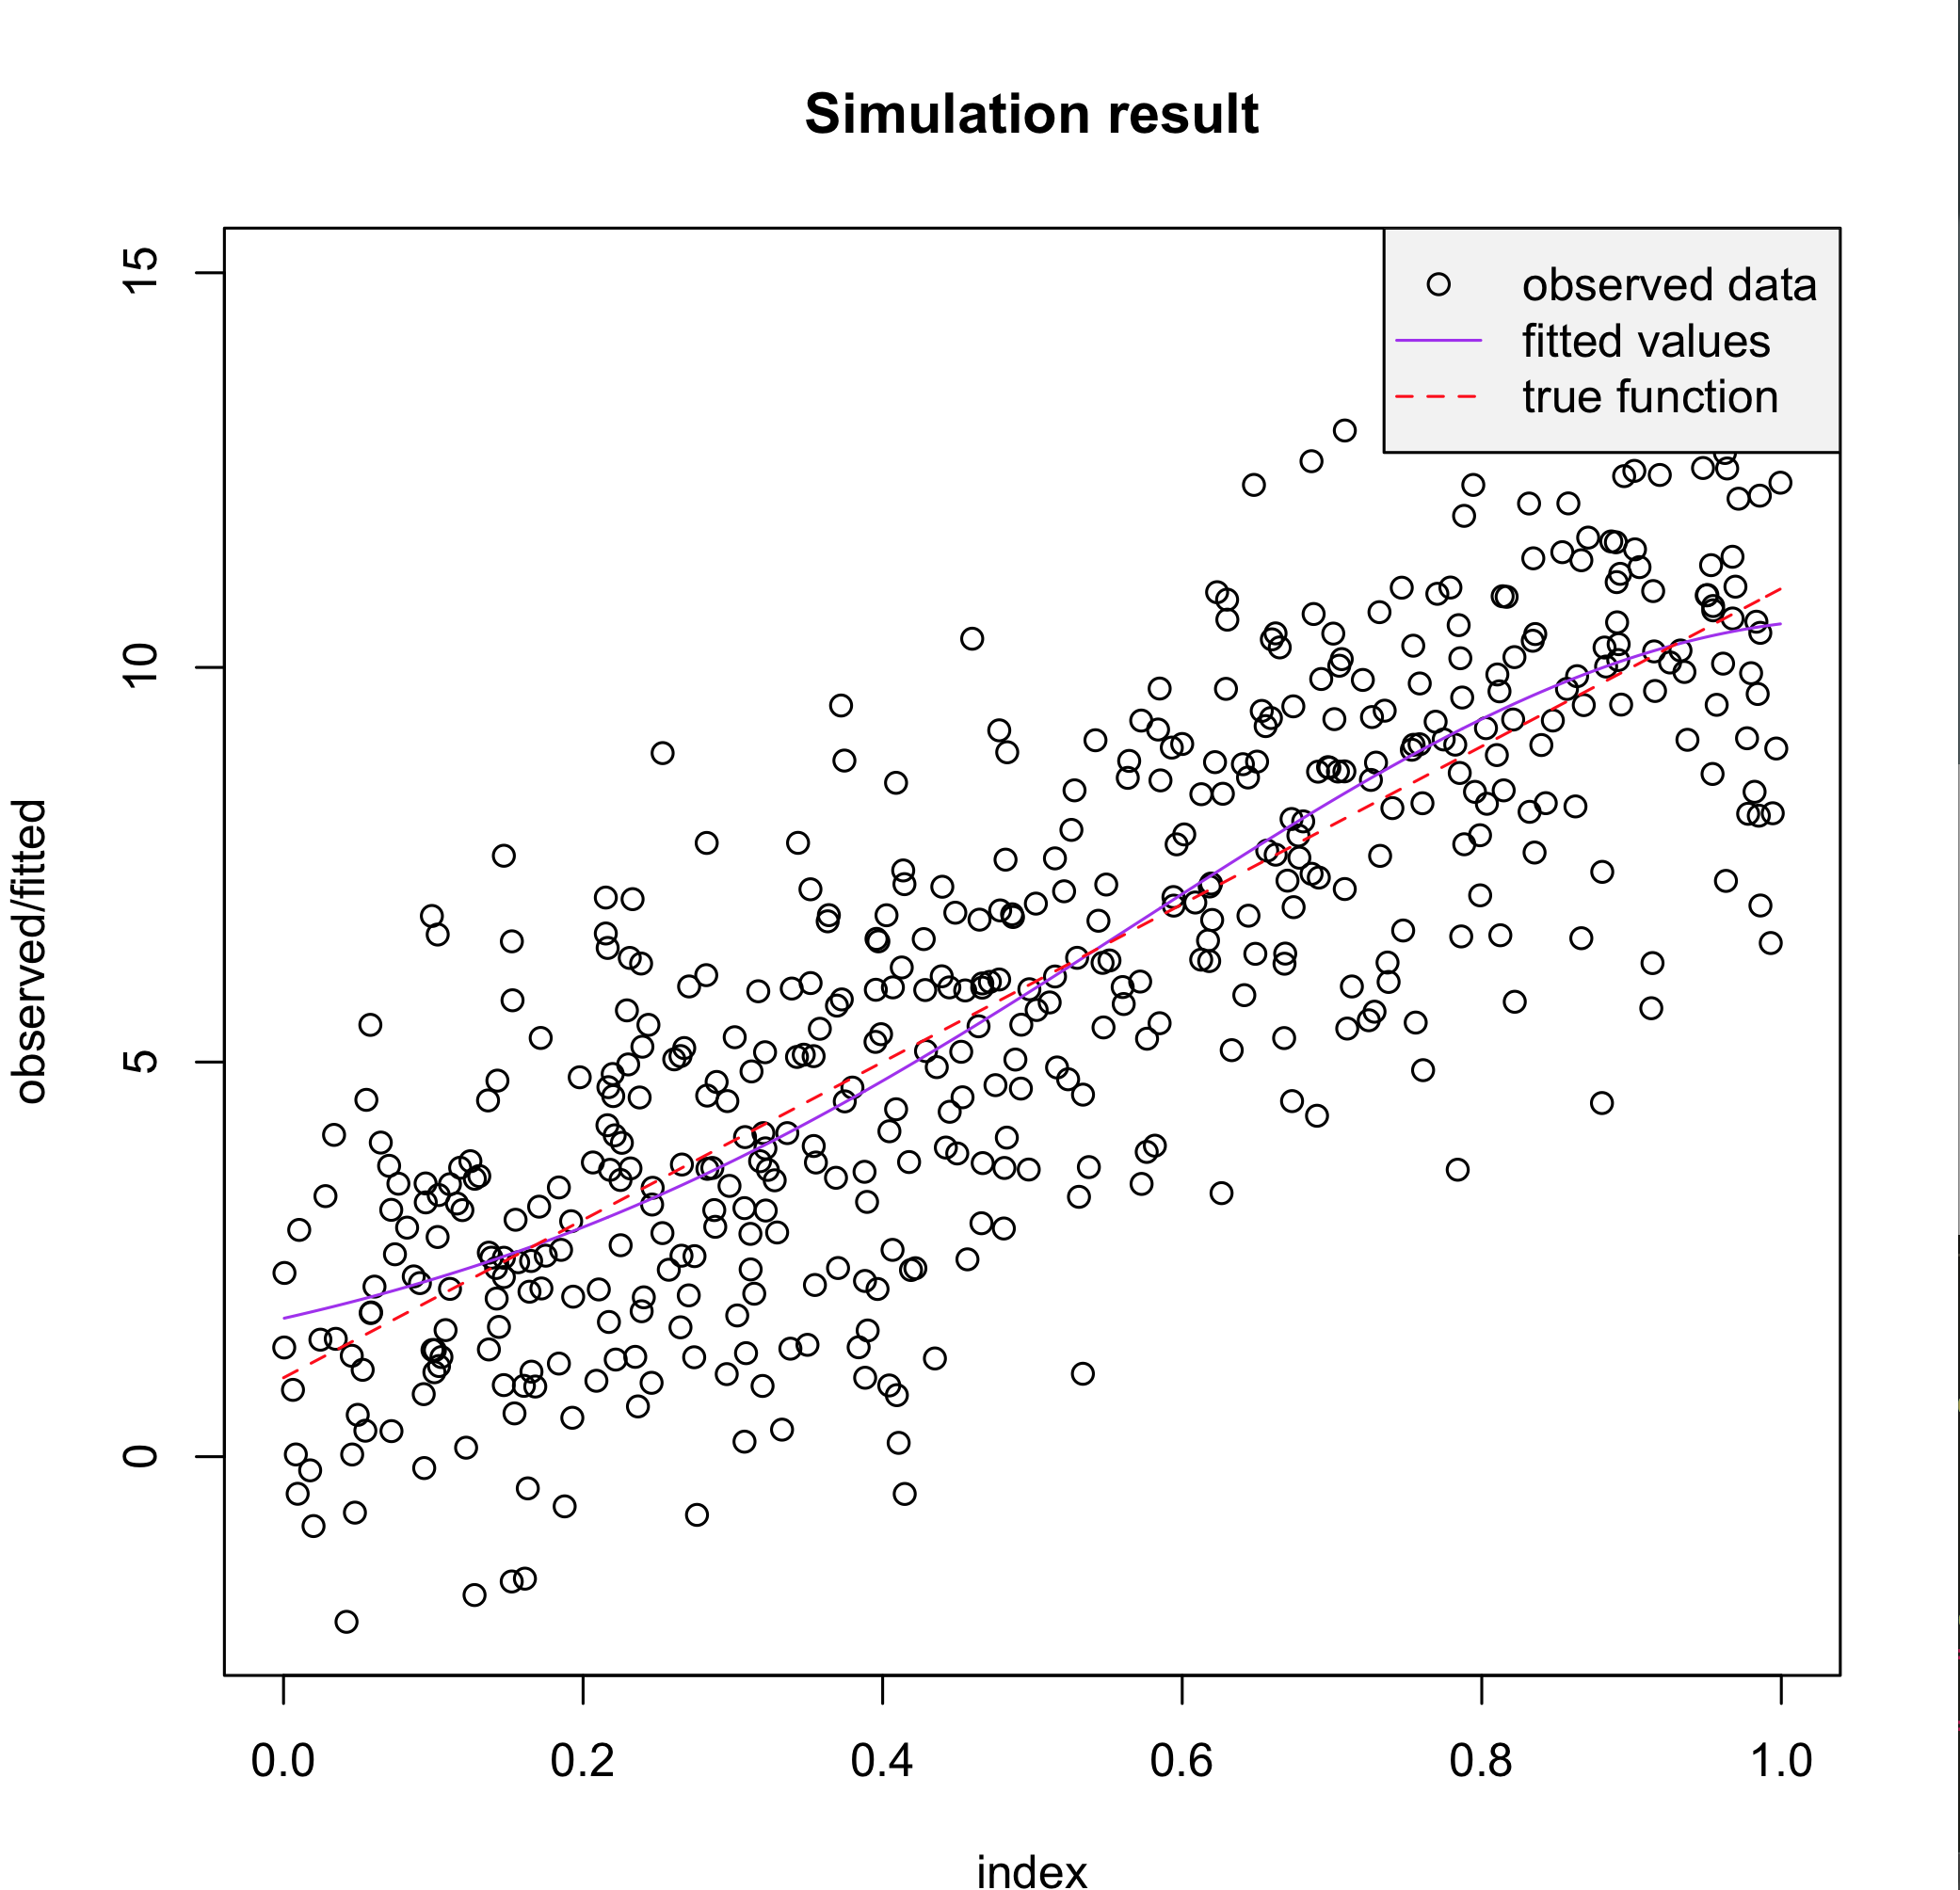
\includegraphics[width=.4\linewidth]{GP_noRE}
      \caption{A subfigure}
      \label{fig:sub1}
    \end{subfigure}%
    \begin{subfigure}{.5\textwidth}
      \centering
      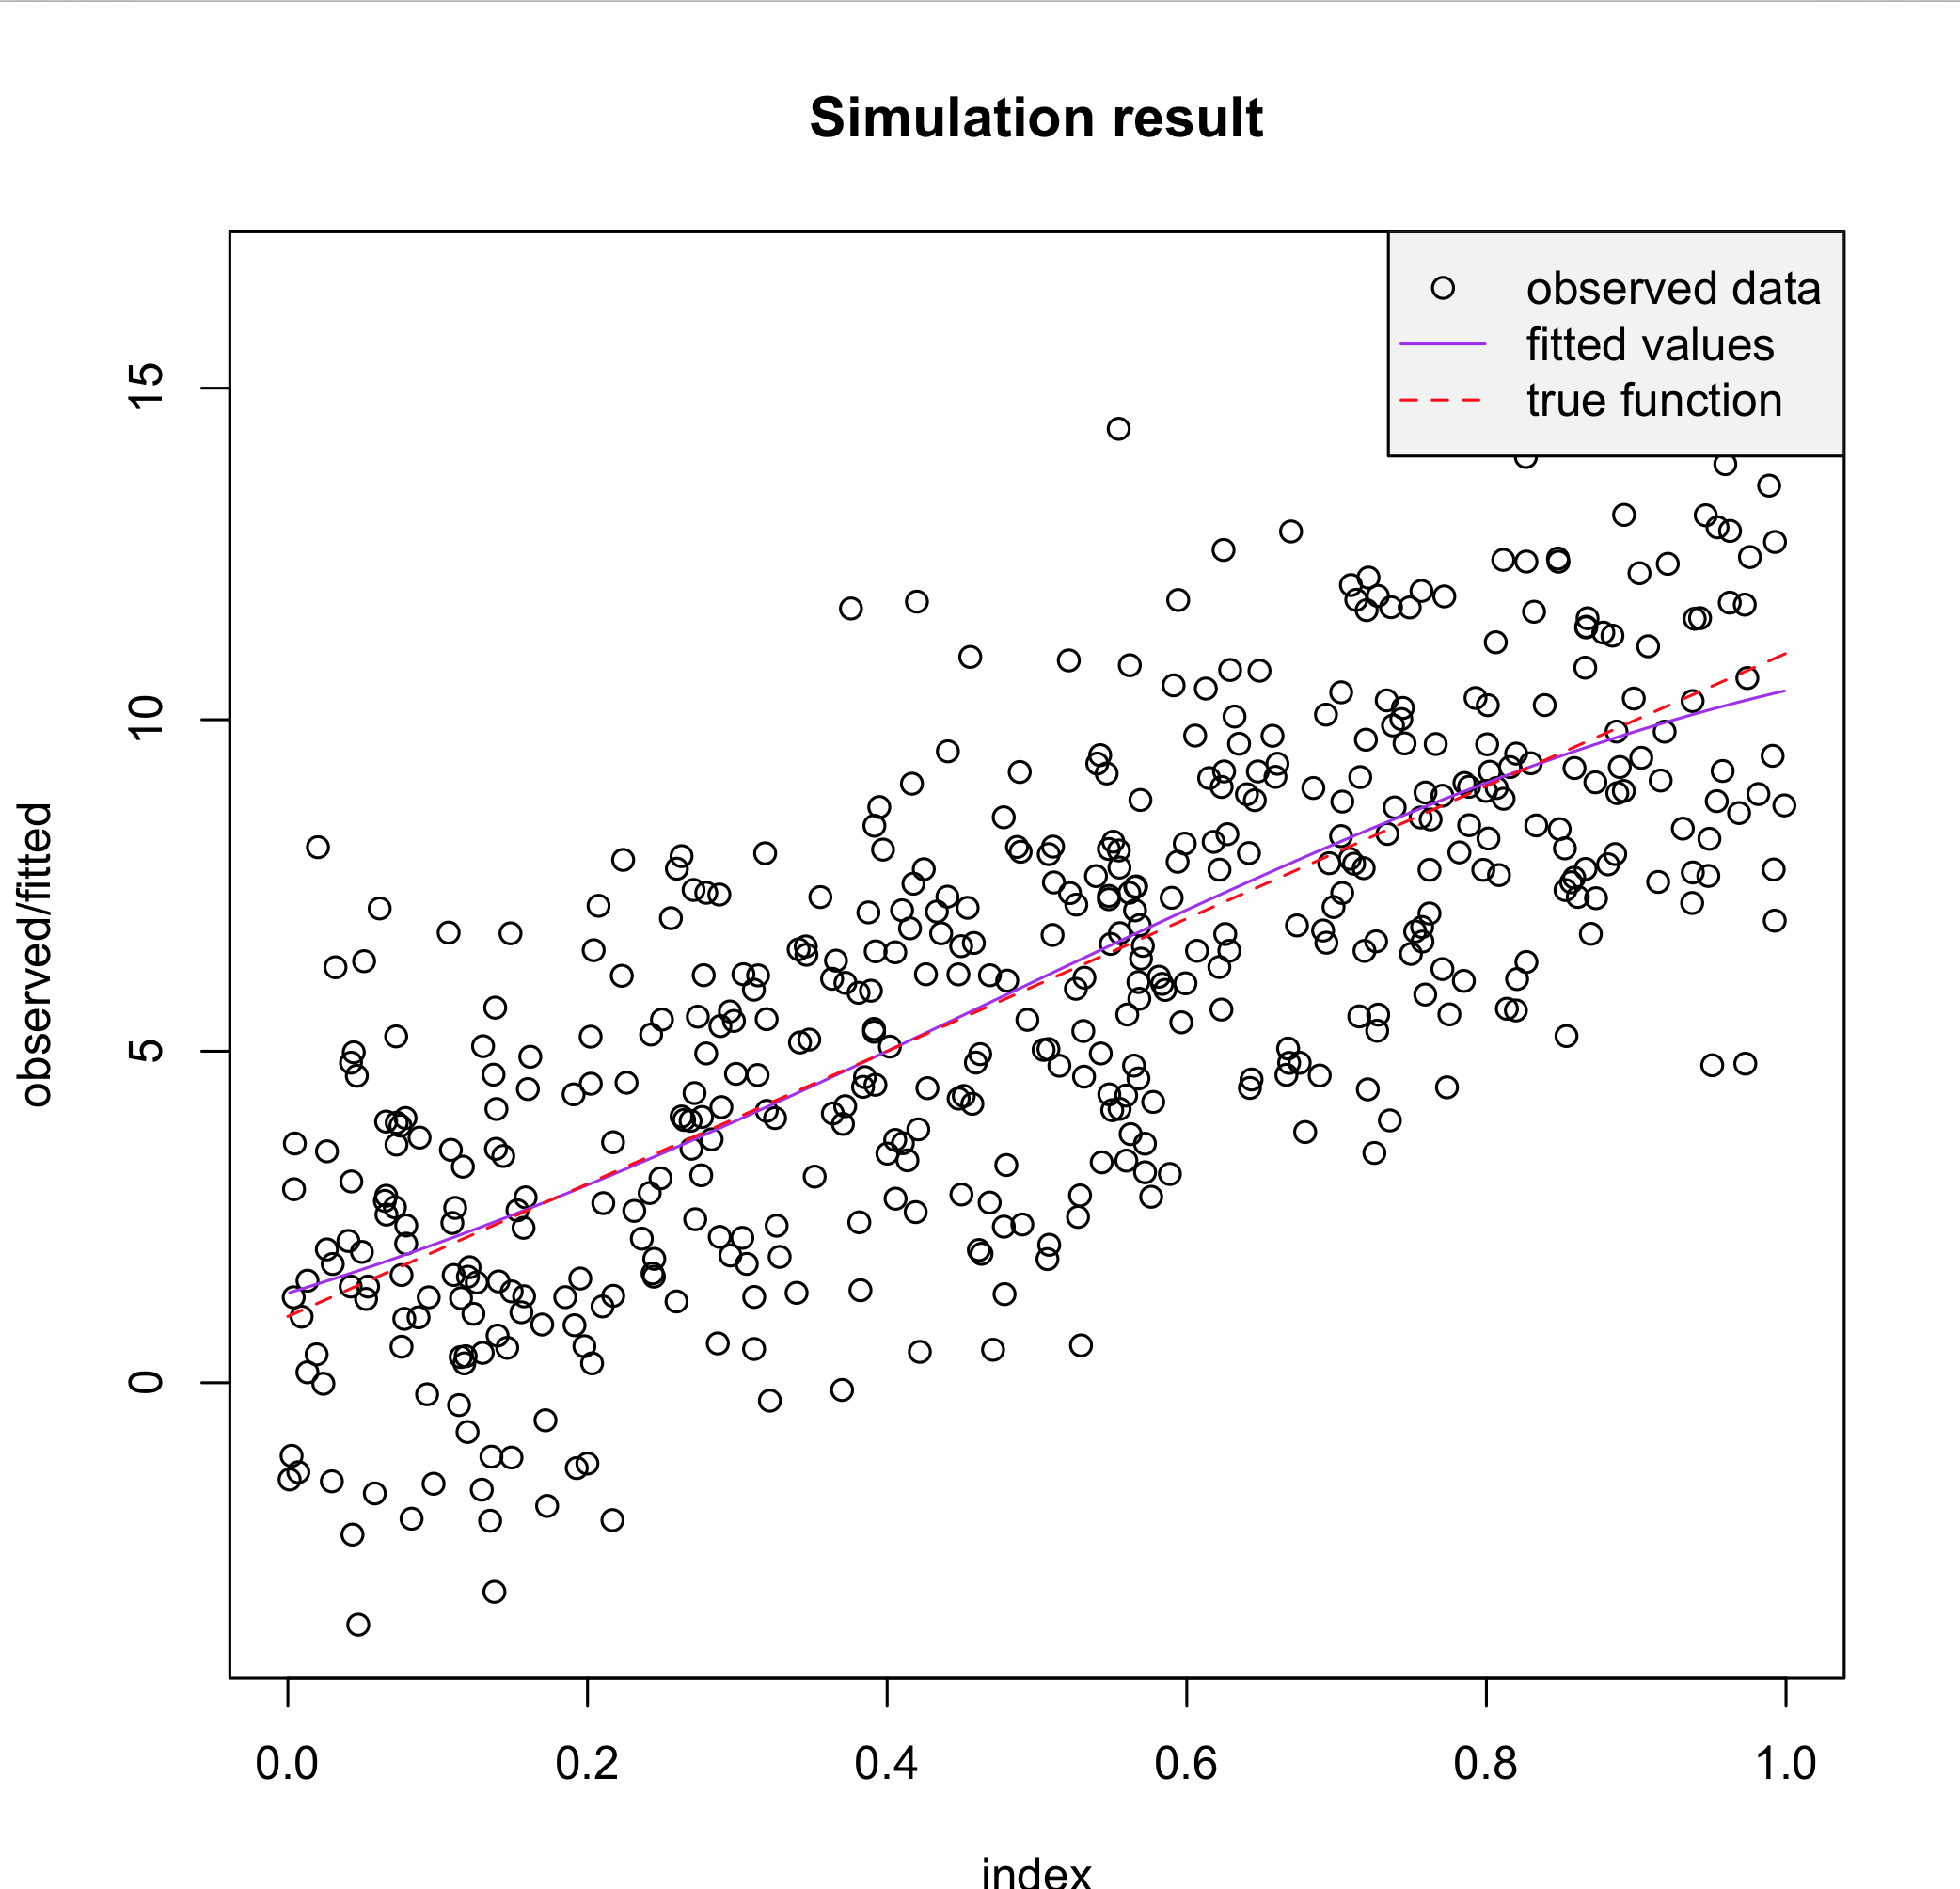
\includegraphics[width=.4\linewidth]{GP_normalRE_linear}
      \caption{A subfigure}
      \label{fig:sub2}
    \end{subfigure}
    \caption{A figure with two subfigures}
    \label{fig:test}
    \end{figure}

    \begin{figure}
    \centering
    \begin{minipage}{.5\textwidth}
      \centering
      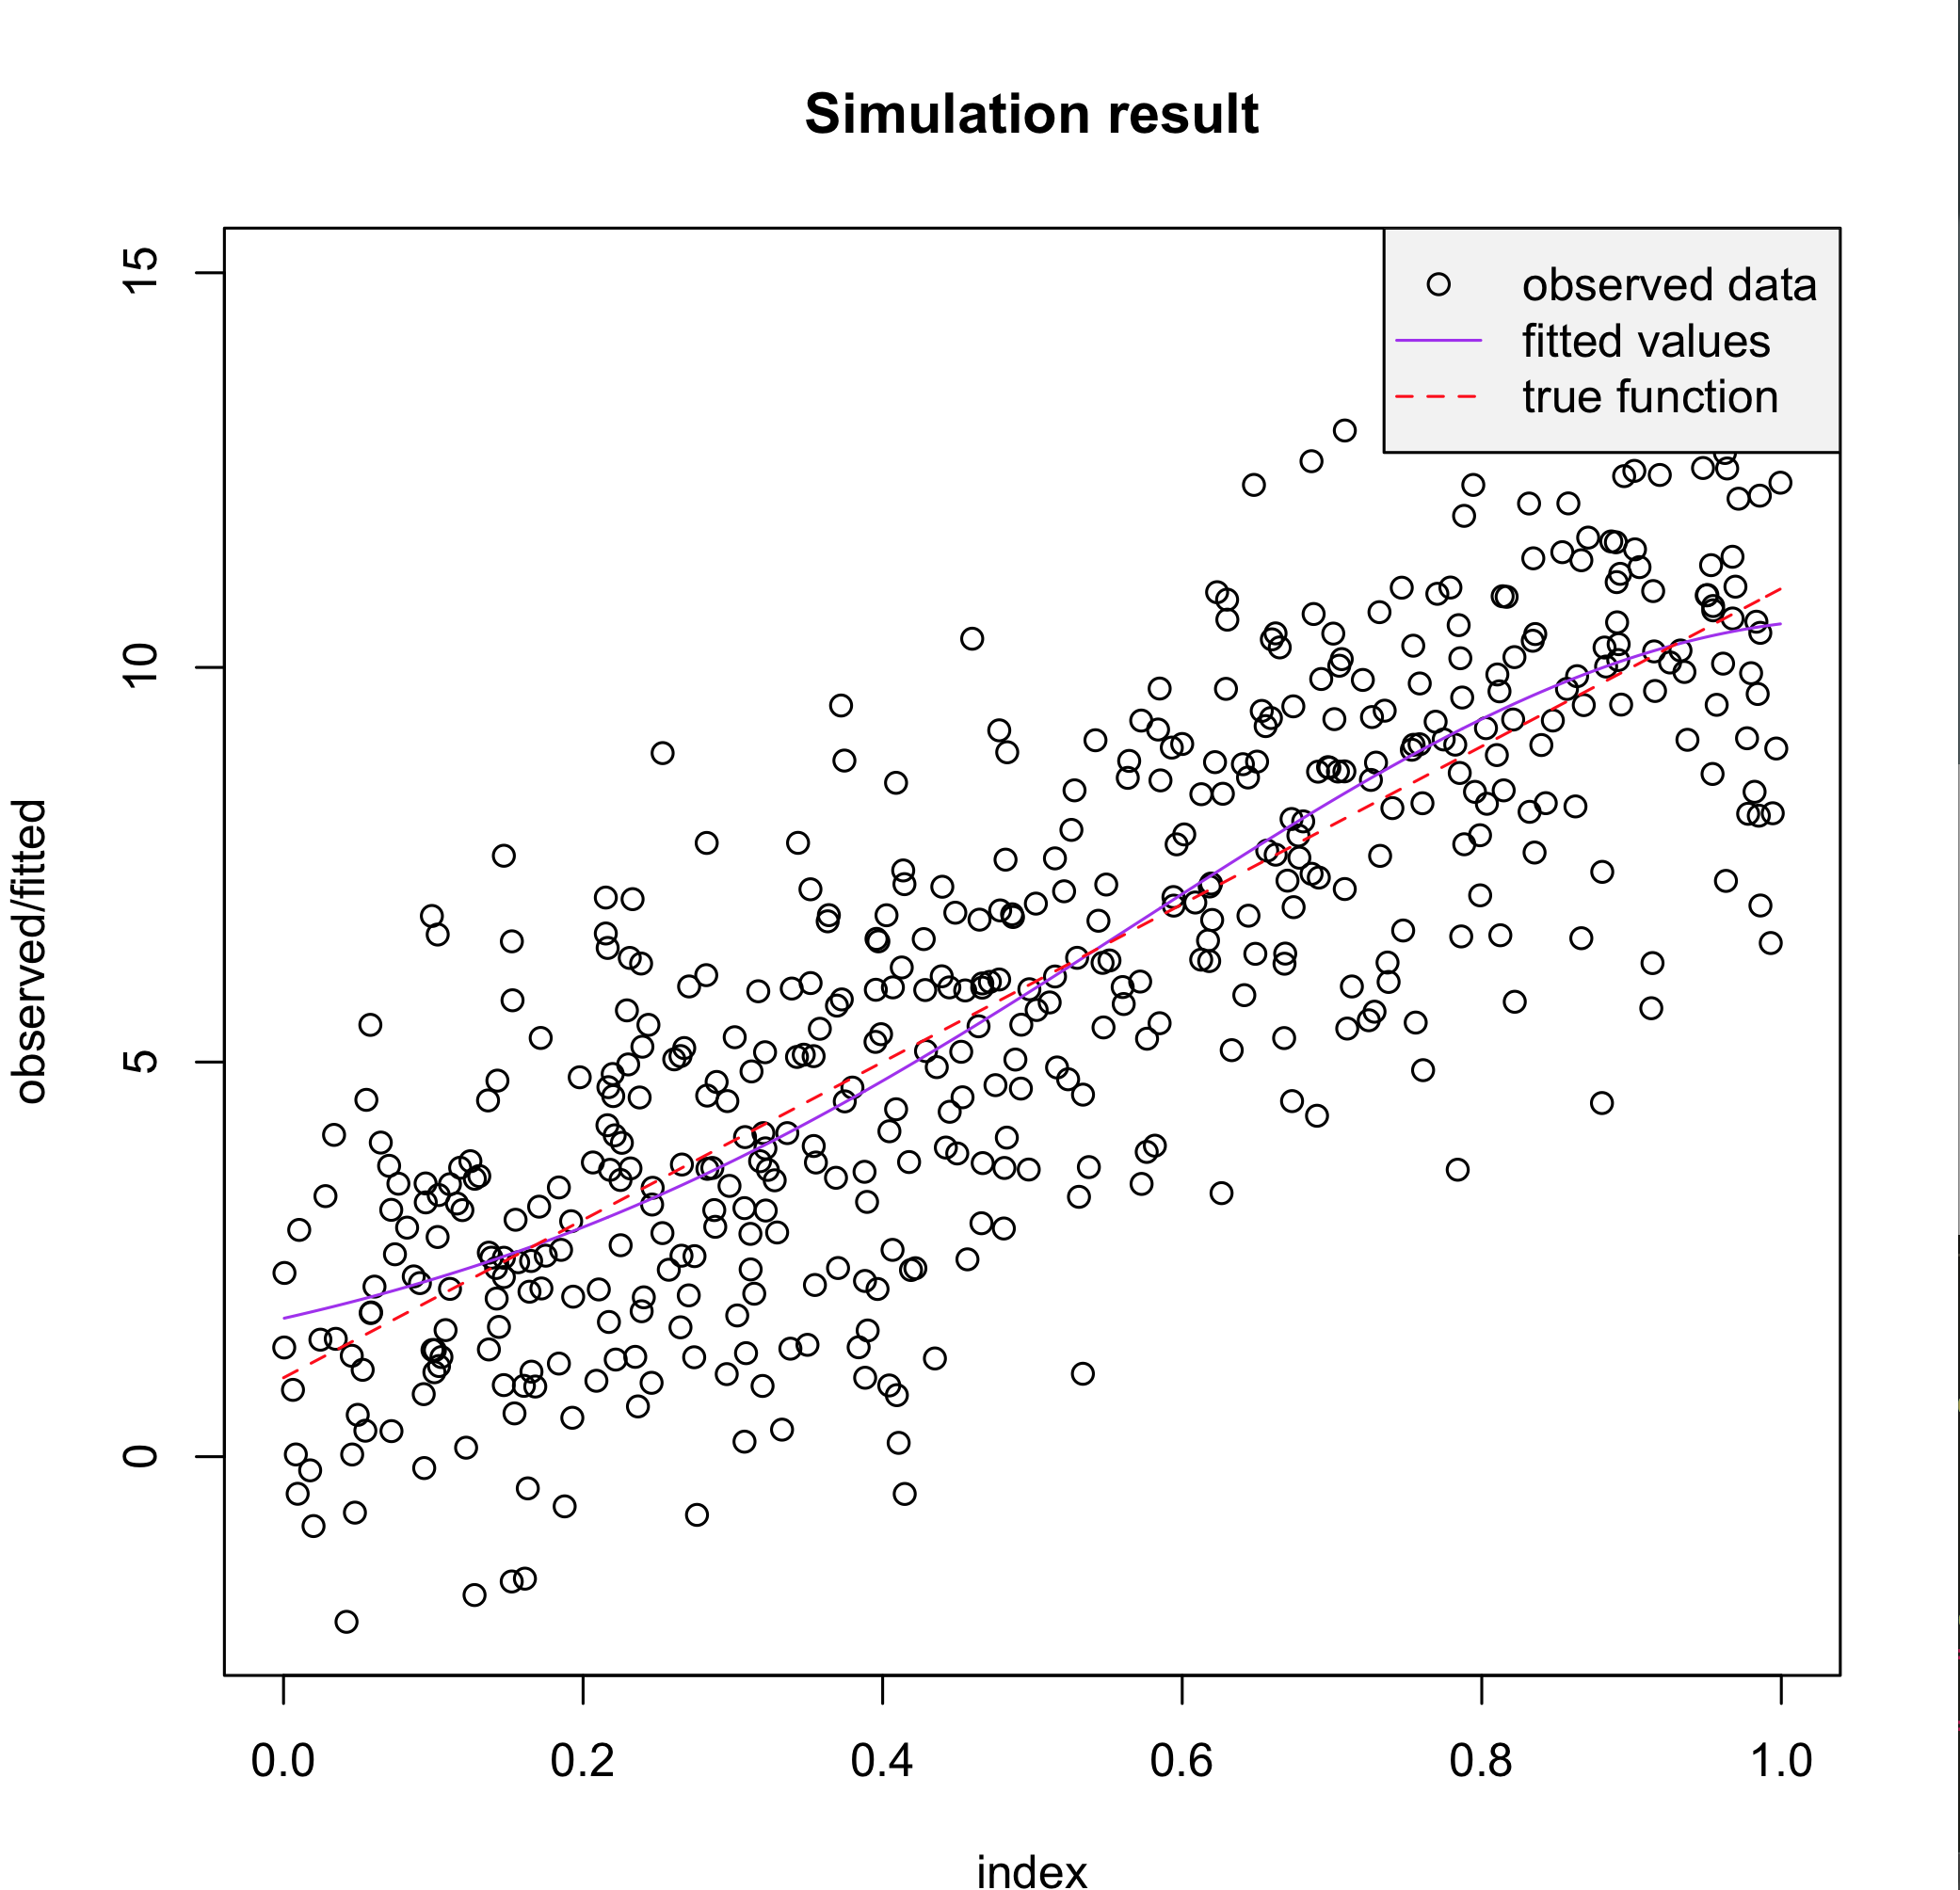
\includegraphics[width=.4\linewidth]{GP_noRE.png}
      \captionof{figure}{A figure}
      \label{fig:test1}
    \end{minipage}%
    \begin{minipage}{.5\textwidth}
      \centering
      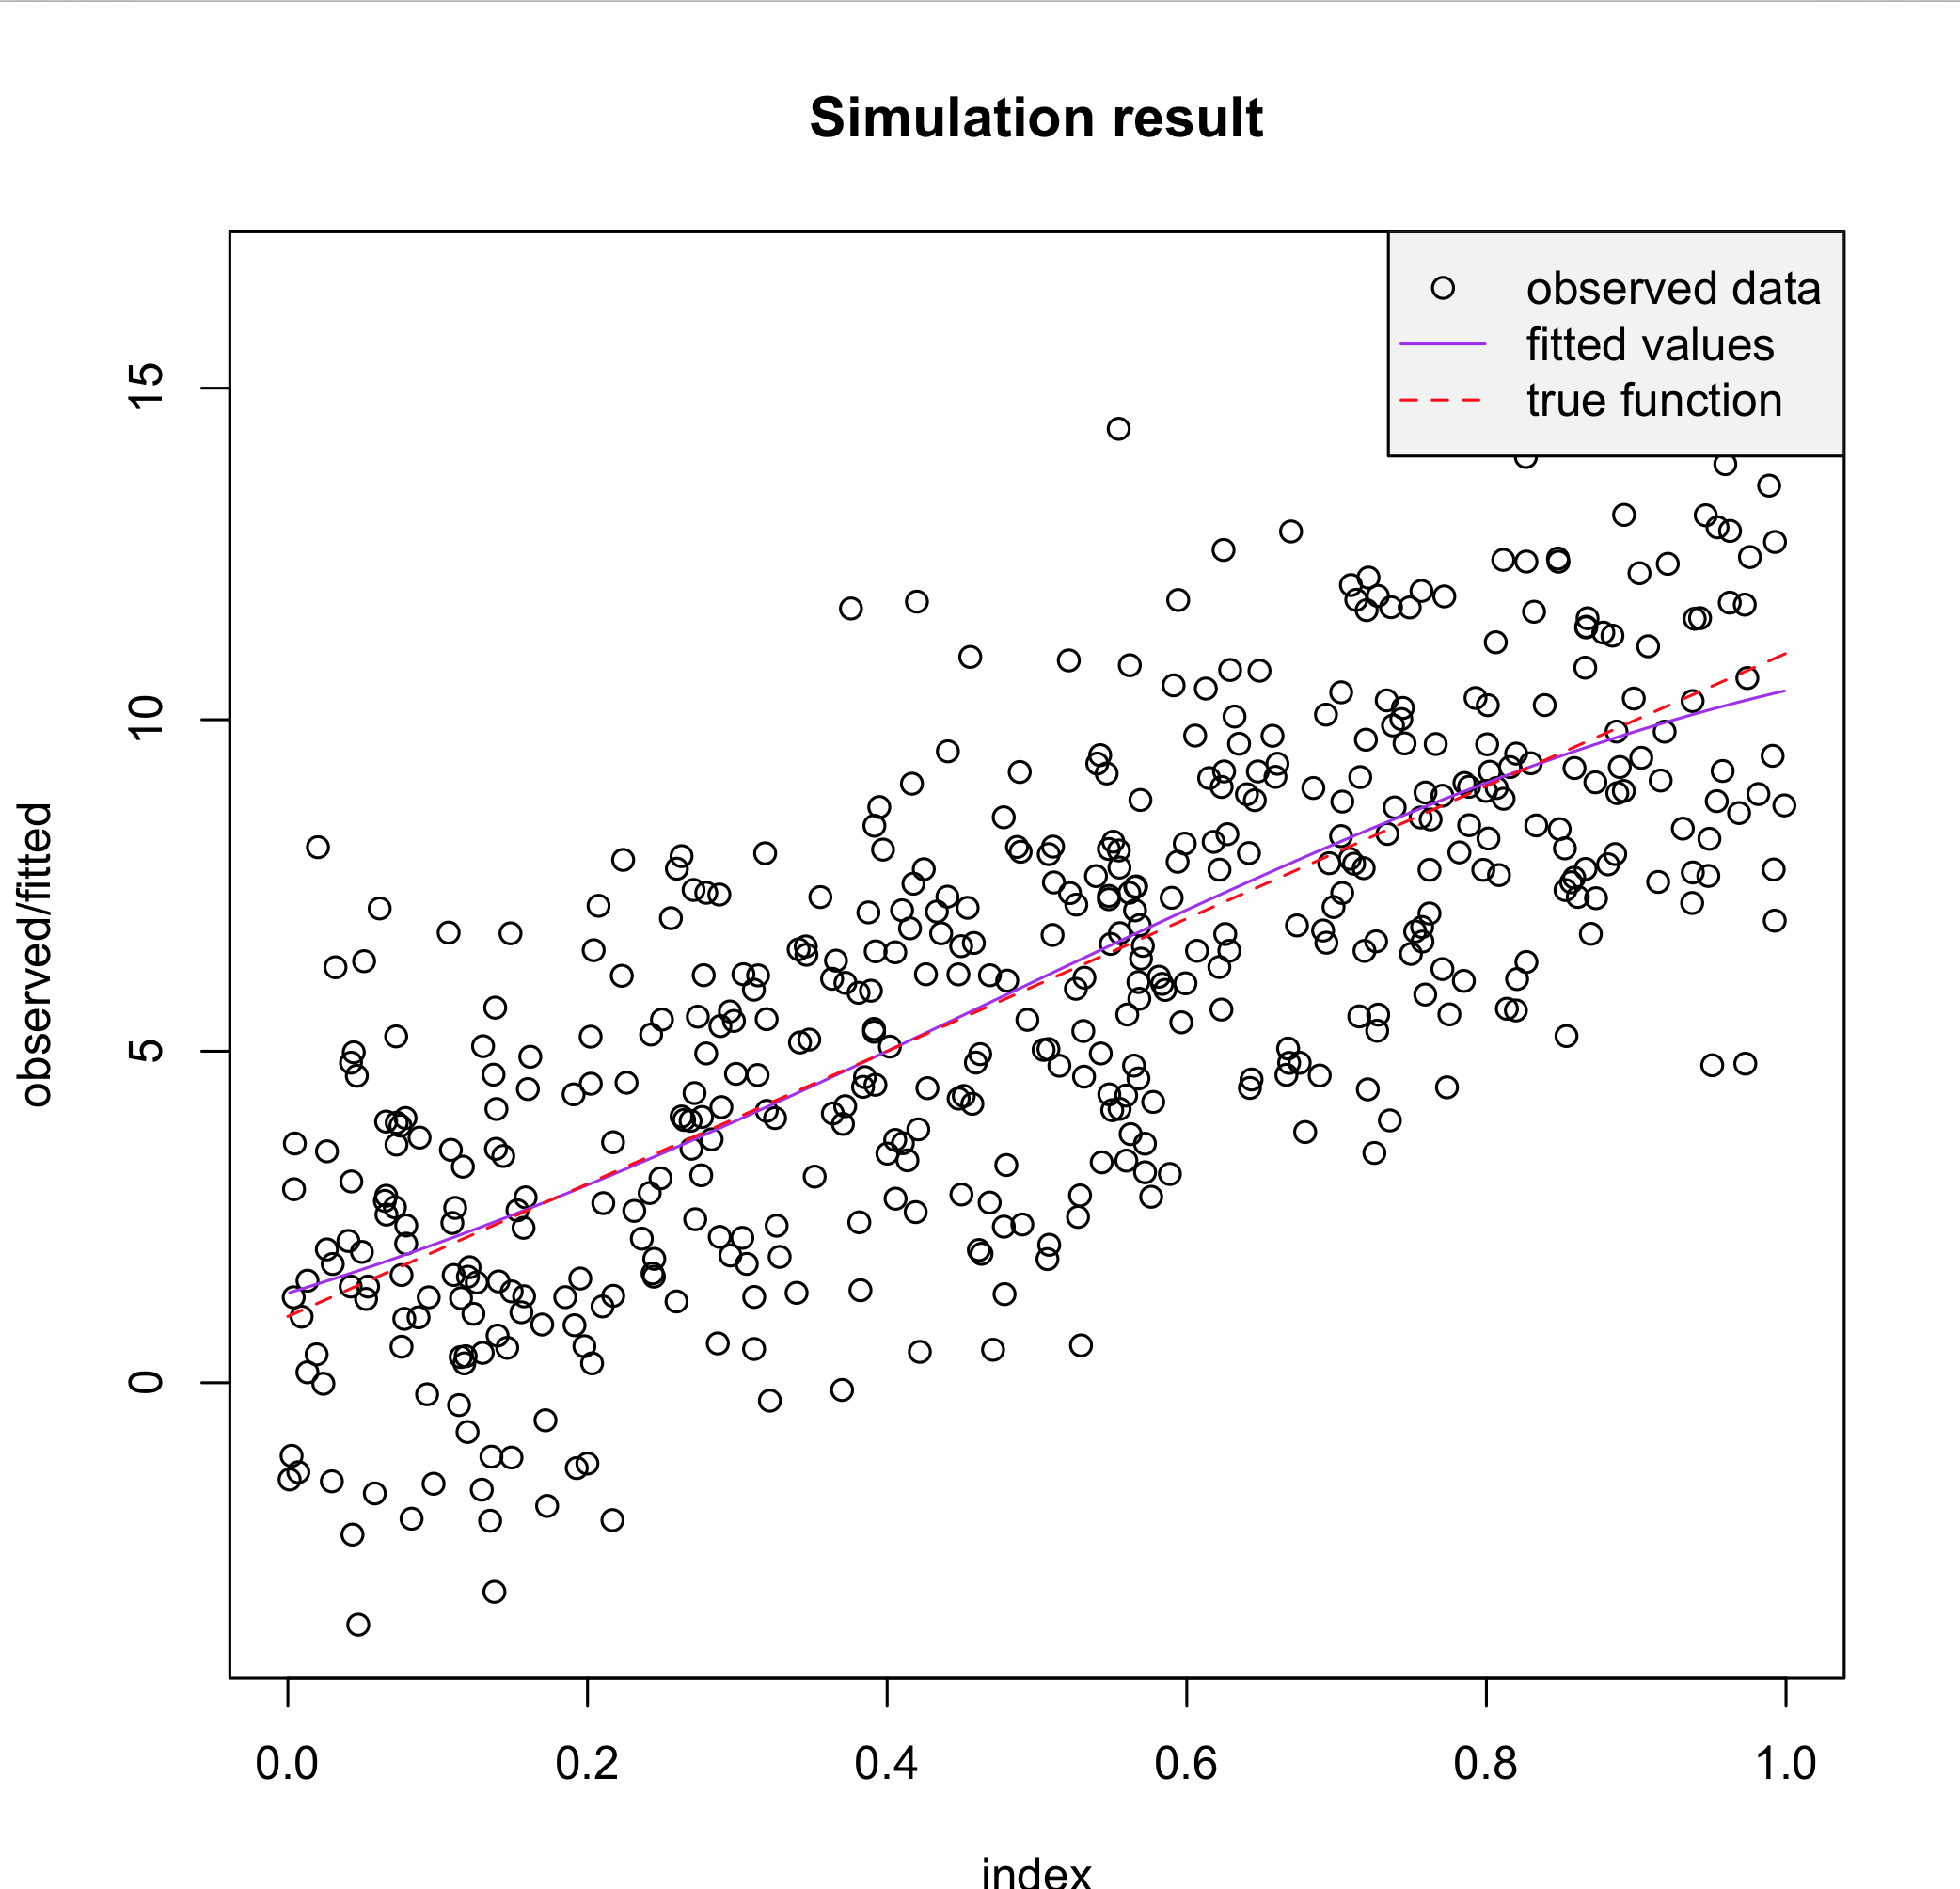
\includegraphics[width=.4\linewidth]{GP_normalRE_linear}
      \captionof{figure}{Another figure}
      \label{fig:test2}
    \end{minipage}
  \end{figure}

\end{document}